\documentclass[journal]{IEEEtran}
\usepackage[english]{babel}
\usepackage{graphicx}

\begin{document}
% can use linebreaks \\ within to get better formatting as desired
\title{Collision avoidance for robot swarms focused on maneuvering and data collection rate from a RTOS approach}

\author{Yu~Shan~Hsieh,~\IEEEmembership{Engineer,~Hewlett Packard,}
	Ignacio~Garita,~\IEEEmembership{Engineer,~Hewlett Packard,}
        Horacio~Hidalgo,~\IEEEmembership{Engineer,~Hewlett Packard}%
\thanks{}%
% The paper headers
\markboth{Journal of ITCR, April~2013}%
}

% make the title area
\maketitle

% in the abstract or keywords.
\begin{abstract}
The ability to convey critical information promptly and efficiently between robot
swarms is critical in collision avoidance scenarios. Different approaches to data collection
are important considerations that must be taken in Real Time Systems where different “units” must
effectively coordinate spatial movement to prevent collisions. Through the use of the computer
networking concepts such as the multicast protocol, our team has devised a new method for
data collection in order to meet the timing constraints of a dynamic system such as this. The multicast
concept allows for information management and establishment of policies related to a set of
subscribers to a particular multicast group, which receives messages from a spatial element who
manages and coordinates information and policies between the subscribed elements. The dynamics
of different multicast groups (of which a single subscriber can be a part of many) creates localized
information hubs and information that need not be distributed across entire networks. The resulting
hubs are flexible, sometimes redundant, localized environments that have better adaptability
to the immediate surroundings. Future studies and application of this networking concept can
provide legitimization of the algorithms presented here; for example, use of robots swarms in an
environment which is not homogeneous and where subscribers will obtain only relevant information
to a specific area of this environment.
\end{abstract}

\begin{IEEEkeywords}
MCAST, collision avoidance, RTOS, data collection, manuevering.
\end{IEEEkeywords}
\section{Definitions}
\begin{itemize}
\item QoS - Quality of Service
\item delay - in networking is the time elapsed from the moment a information is send to the moment in which it is received. For the interest of this investigation the case is extented from the moment the data that produced such data was sensed to the moment in which the information was processed in the destination.
\item jitter - is a variation in the delay of packets arriving at the destination for a received data stream
\item Multicast - A layer 3 protocol part of the TCP/IP stack used to send information to multiple points with just one data transmission
\item MCAST - Multicast
\item DMA - Direct Memory Access
\item EDF - Earliest Deadline Fist, a scheduling algorithm that gives the priority to the task whose deadline is the closest.
\item UAV - Unmanned aerial vehicle
\item RTOS - Real Time Operating System
\end{itemize}

\section{Introduction}
\IEEEPARstart{A}{d}vances in technology have allowed automatons to gradually replace humans in many tasks involving control. Automated spacecrafts and UAVs (Unmanned Aerial Vehicle) are being heavily deployed in todays military operations and the scientific
community uses unmanned spacecrafts in space explorations. Although these automatons are usually expensive and sophisticated, more economic solutions are now being used in civilian applications \cite{YS1}.

Well established engineering technologies have been made for these mobile UAVs to move around as a single unit and most of the time you will see a military drone fly alone to strike its target and then escape without being traced. Or a single spacecraft wandering over the surface of Mars and other planets. And rarely if not never will you see more than one Google vehicle cruising through the streets and roads to map every block of the city. Will the era of large fleet of planes like those of World War I and II one day return? Back in those times, large formations of planes consisting of many light fighters would often accompany a few large bomber in its bombing mission. Should a hostile plane come into the area to take the bomber down, the fighters will break formation, attack the intruder and return to guard the bomber. Such behaviour could be done by a swarm based on similarities to the movement of a swarm of bees or a flock of birds. Popular culture \cite{YS2} in television and science fiction forsee the return of these swarm-like formations, often depicted in the form warplanes and spacecrafts using it's advantage in numbers to spam and overwhelm the opponent. Returning to the present real world, imagine a large fleet of unmanned spacecraft moving in a formations across Mars; if one or few vehicles stumbles upon a large obstacle such as a lake or a crater, it can quickly inform the other spacecrafts behind him to detour and find another route. And if one of the spacecrafts breaks down or gets stuck in a mud-like terrain, other spacecrafts close to it can assist him in getting out. Currently, there are already similar projects in the way. Started in 2010, the MIT developed a fleet of low-cost autonomous oil absorbing robots to help out during oil spills \cite{YS3.5}\cite{YS3.6}. Dispersion and quantity are it's main strengths. 

If the "robots" in this case scenario were to be exemplified as computers each with an operating system inside, it would require an RTOS (Real Time Operating System) to manage all its tasks as it exhibits all the characteristics that calls for an real-time solution. Stankovic \cite{YS3} argues that these systems must be:

Although there are lots of applications that might take advantage of the swarms in order to make productive jobs, there are day to day applications that are practical and could allow a practical approach inmediately there are already traffic assisting software tools to provide best time routes but the actual information shared by users is very limited and the technology used by the vehicles is not though as it could be take advantage of these type of information, meaning there are limitations needed to be overcome but if proved and quantized advantages improve energy efficiency, increase route capacity for highways or aerial routes, save time and finally increase the reliability and safety of the vehicle fleet.

\begin{itemize}
\item Fast.
\item Predictable.
\item Reliable.
\item Adaptive.
\end{itemize}

For this paper, we will delimit the use of real time system in the context of the robot's maneuvering and data collection system to allow the robot to move freely without human intervention while preventing collision with obstacles including other units of the same type. It will focus solely on conceptual aspects and ignore all implementation considerations. 

Additionally, there are some assumptions that are taken:

\begin{enumerate}
\item The spatial location is determined using 3-dimensional coordinates.
\item The units have a defined radius of communication.
\item All tasks are dynamic and aperiodic.
\item The arrival of the tasks are sporadic in nature.
\end{enumerate}

In this paper, we will start off by discussing various concepts pertaining RTOS and how it applies to our model. We will also describe the use of Multicast protocol to improve the performance of the real time solution. The first part of this paper covers various concepts and definitions related to this subject. The second part describes the test we did to simulate such model. Finally, we will summarize our findings in the conclusions and discuss the advantages and disadvantages of such implementation.

This paper makes the following contributions:
\begin{enumerate}
\item it presents a problem that requires real-time solution.
\item it presents a novel solution to reduce the amount of information to handle.
\item argues the importance of reducing information to process to meet the timing constraints.
\item it presents a simple experiment to prove these ideas.
\end{enumerate}


\section{Research}
\subsection{RTOS}
A control unit responsible for the movement of any unmanned vehicle is constantly handling inputs from sensors to get information like the current speed, acceleration, the direction it is heading. It must be able to detect near term obstacles and perform various tasks like computing the shortest path, the amount of energy it needs to inject to keep the current velocity, etc. As such, it require a time sharing notion from a operating system's standpoint. Apart from being time sharing, the tasks have different priorities among them. There are critical tasks where the very existence of the robot is threatened should it miss its deadline and then there are tasks that can be done in its idle time. These characteristics makes it a suitable candidate for using a real-time multitasking operating system.

Real time operating systems can be divided into four classes depending of their characteristics; they can be Static or Dynamic, periodic or aperiodic. In this case, we can assume in the worst case that the task is dynamic and aperiodic meaning that the tasks are constructed in runtime and the arrival times of the tasks are not constant, in fact, they can be sporadic. An example of a sporadic task would be the obstacles encountered by the vehicle along it's path.

Multicast constrained by QoS routing its by itself NP problem usually resolved by Heuristic approaches \cite{HH1} which its optimum performance is assumed out of the scope of the paper but the approach to  intercommunication between individuals of the swarm is by multicast relying on the network infrastructure to take care of the communication paths leaving to the individuals the task of just establishing the connections although Jin Lul et all. \cite{HH2} propose ad hoc networks across the individuals of the swarm having them as retransmission stations and having needs for processing of information in real time.

The focus of this work is on using multicast as a source outside of the swarm like a control tower works for a airport or the cellular towers work for Internet access to information like real time traffic reports\cite{YS1}

\subsection{Collision Avoidance}
Collision avoidance is a reactive action based on information sensed from the environment without which a collision would be determined to happen. It is an inevitable problem for swarm robots; they must avoid collisions with moving obstacles, other robots within the swarm and static obstacles. Control policies and strategies \cite{IG6} are needed to avoid collisions. 
Elements of collision avoidance
There are many elements that need to be taken into consideration for a robot to adapt into its environment and act accordingly to the dynamic stimulus it must receive as it interacts with the environment. The robot must be able to adjust its behavior due to many types of variations. For collision avoidance a central problem are velocity vectors, acceleration \cite{IG9} robot orientation \cite{IG7} and mass. Synchronization \cite{IG8} is also a relevant characteristic that can be modeled mathematically \cite{IG8} to regulate flock centering and direction and collision avoidance.
Real time considerations are also relevant; robots must take decisions in real time to avoid a collision. 
Another set of elements used today in this field are development of sensor technology, communication technology , artificial intelligence; all maybe part of swarm robotics and help create greater robustness and adaptability for robot swarms.
Thus a key and central part of collision avoidance has to do with the collision avoidance algorithm, and which elements it responds to. The algorithm must be able to prioritize actions to avoid collision.  Multi-agent swarm algorithms have been already developed for swarm systems \cite{IG10}. Ye Wang, Tanaka and Guan \cite{IG10} develop interesting association (called dynamic association) algorithms based on “light of sight” or robots not obscured by obstacles to associate different robots within themselves (this is interestingly the closest implementation similar to multicast found in our research). In general this is just an example of how different algorithms can be used to implement collision avoidance techniques. In our research and experimentation, collision avoidance was modeled only based on proximity; other techniques and capabilities are left for further research.

\subsection{Data Collection in Real Time}

While this is a topic where only one reference was found that directly relates to data collection in swarms\cite{HH5}. Applications require minimum throughput and maximum delay guarantees, that need to be accounted for in the design, also trajectory planning  and communication-aware route planning has been an area of interest to different robotics and communication communities\cite{HH5}.
It is supposed that the data collection involves a DMA access from a network device involving little to no overhead to the processor, having to focus more on selecting when to process the data and when it is not worth to be processed.
In relation with multicast, in the case of a individual with multiple channel subscription, the number of channels is unknown a priori, each channel or subscription is likely to represent the given amount of individuals in the vicinity of the system. The amount of data to be processed is important for the scheduler to define a window for the validity of the data received based on a more recent set of data arrived from such individual, meaning that what would matter most is the most recent data and once a data set from the individual has arrived the previous data has little to no importance.
Based on closeness to the individual system different multicast channels a priority could be established for each one of the multicast channels that are listened each representing the information about a individual in the swarm like position coordinates, speed, acceleration obstacles found, any planned maneuver or any other interesting information for the other individuals that would help them to take better decisions to avoid any collision.
Other important aspect is the knowledge of when the information received was actually measured or calculated as the network delay should have an impact on the validity of such data at the received time making the information perceived with a error or with the need to actually perform calculations just to compensate the delay, such problem would require a global swarm time synchronization to acknowledge the interpretation of the information at the time of the reception being highly desirable to minimize delays that could cause the additional calculation, and the jitter could actually make this compensation to vary in time adding an error to a compensation that could be calculated esporadically\cite{HH6}.
Given a set of multicast channels of the same level of importance is mandatory that the computation associated with those would be evenly distributed among all of them as such a simple round robin between each of the channels would be fair so that each one gets to process the data set received.
Although was previously shown the data set received contains multiple variables all those which could arguably have a relative higher importance to the system in order to avoid collisions or perform maneuvering, meaning that the whole data set could be processed in parts according to the importance of the data set or seeing from another perspective from the functions operating over those parameters like time to collision, speed variation angle, calculate average direction of neighbors, and obviously the time at which this information was measured meaning that each of the operations could be scheduled with a different degree of importance and a appropriate compensation could be applied to the data.
Once the nature of the data processing is well understood priorities could be given to each of the different functions instead of the different multicast groups.
A fair scheduling policy in these circumstances would have a round robin between each of the critical tasks and have data sets with a time window with expiration once a new data set arrives for the same multicast group.
For speed and simplicity the data processing operations should be made very compact and atomic having data invalidation only after the operation over the data set  has been completed, meaning it would be favorable to have specific data points in which to preempt the system or have a non-preemtive nature of the computation for data collection
An strategy could arise when processing the data as there are certain tasks that need to be done at every cycle and the remaining of the time could be used to process information from multicast subscriptions as there is time taking multicast data processing as the server technique used for aperiodic task processing with rate monotonic
After the data has been processed, a decision has to be taken in order to allow the system to correct or make any adjustments as in any control loop, this should be done once a data set has been invalidated or the whole data set has been processed then a higher priority task arises that computes the data computation from the coming data, takes the decision and afterwards the decision must be executed meaning the system trajectory should be adjusted.

\subsection{Maneuvering}
Maneuvering should be understand as a proactive action planned based on information received by other individuals or by simply knowing a priori that a certain maneuver has to be done at a certain point in the route like taking an exit in a highway for a vehicle.

Individuals could be in various states depending on their relationship with a swarm, SingleSearch, SwarmSearch and Declaration according to Tang Ying \cite{HH4} as is likely that individuals would like to join a swarm if they are alone, so a comprehensive research on the search of swarms by an individual could be found there.

Other assumption is that individuals have particle properties, meaning they could have infinite acceleration, no inertia nor speed limits \cite{HH4}, although in the experiment the speed was assumed to have discreet values, in particular a single positive speed and 0 or static.

There could be distinct types of maneuvering, for example thinking in the context of vehicles in a highway they could have a particular destination, they might want to be part of the swarm or a group of vehicles for optimizing energy consumption as they packet could be more fuel efficient, in such scenario vehicles join and leave the pack as their paths collide or diverge with the swarm, there is critical information that is needed to be shared for other individuals to take actions, like yield when a new individual is incorporating to the pack and same when it is leaving so that those transitions are smooth and does not require a quick and dangerous action as long as the affected individuals which are close to the one differing with the swarm movement are notified of the maneuver ahead of time so that they could take smooth action proactively.

\subsection{Cross Applications}
An underlying realization product of the problem we set out to answer is that cross-applications of other fields can have interesting and unknown results. In our case multicast has no similar applications in the industry or research areas. First, there are possible applications of our use of multicast in other real time systems related to swarms, and for different types of swarms. Second there are many possible applications of networking concepts in many other areas, and it is possible that they may be applied in other types of swarms as well. 
This let us to think that our research and experimentation definitely support further research in this area, and a basis for an expansion of the current research to yield more conclusive results. 

Our research in the available publications and papers indicate that that few if any (none were found) groups or individuals have used a computer networking protocol such as multicast applied to a robot swarm problem to specifically manage behavior (and ultimately communication) between swarm robots.
Most of the articles and papers found related to robot swarms contain information about using robots swarms, particles or swarm intelligence to improve and optimize the multicast protocol \cite{IG1}\cite{IG2}\cite{IG3}, but not for the inverse relationship, were a networking routing protocol is used to improve robot swarms interactions. 
Not only is this promising because it is a novel idea that can be applied to other fields, but because there are still many networking protocols that can be used for exploration and improvements in robot swarm behavior (or other behaviors and problems). 
This let us to think of the substantial value of cross-applications of systems, methods and practices used in a field, applied to another field. A clear example of such a cross-application is the biomimetics field, where biological systems are used as models for design of machines or engineering materials and principles. Other clear examples include neural networks, ant algorithms, genetic algorithms; all which are used in the computer science field successfully (and ironically can be used to improve the multicast protocol itself \cite{IG1}\cite{IG2}\cite{IG3}). 
Computer networking protocols and routing algorithms can be cross-applied to other fields. Many of these algorithms and methods have been modeled to efficiently manage packet data across networks, of which multicast is only one of them.  There are many other protocols that can be cross-applied in an interdisciplinary fashion. The computer networking area is a mature field that has evolved and is used today as the basis of many Internet networks. It is possible that many of the elements of such a system such as meshing, spanning tree, policy based forwarding, tunneling, congestion avoidance (to name a few) or other capabilities of networking be applied to robots swarms or any other fields that may warrant an intelligent reuse of these concepts.  Our study and our application of the use of multicast can be a starting point to a) further use multicast with more parameters that define the application of multicast. Our experimental application of multicast only takes into consideration the value of proximity; based on proximity robots belong to a multicast group. Other parameters can be used, for example types of robots, types of environments, or any other qualities that will serve as a criterion from which to define subscriptions to a multicast group. The second interesting application derived from our research is b) further applications of networking concepts such as the already mentioned (spanning tree, meshing, etc.) to similar problems. These concepts of a networking system need only be explored and analyzed in a similar way biological systems are used and applied by biomimetics into other fields. 
Furthermore there are benefits of having such concepts that can be described as digital concepts. These are conceptually already modeled in the computing field, and as such are easier to implement as programming models. 
Another strength is that networking tools and systems to analyze networking data and behavior are already present and used to simulate networking behavior. These are known problems with a longstanding in the computer science and telecommunications field, such that there may be a use of tools \cite{IG4} and suites that can be adapted or used to model the possible behavioral cross applications of these concepts.


\subsection{Benefits of application of multicast}
Through the use of a multicast algorithm applied to a robot swarms, the conclusion arrived is that multicast provides a possible reduction on robot swarm transmission of data and information within members of the swarm. Since our experiment and simulation is at this point a testbench with a very small and limited number of simulated robots, the results are not strongly conclusive, but work as an introductory work in the field.  
Regarding collision avoidance, an improvement in data reduction yields a direct improvement in collision avoidance for two distinct reasons. 
\subsubsection{Collision reaction time reduction}
One, since multicast reduces the amount of data to be processed (significantly) by a single entity of the swarm, it has the potential to reduce the amount of reaction time to reduce a potential collision. This is an important contribution in real time systems, where any possible improvement regarding reaction time must be efficiently incorporated into new systems.
\subsubsection{Collision Prevention}
Second, the ability given by the behavior of a robot swarms under multicast groups, where robots are subscribed to other robots according to relevant data, provides an interesting way to prevent collisions. To further explain, in a networked robot swarms such as those described in \cite{IG5}, there may be obstacles that do not warrant an immediate action from the acting robot to avoid collision, but do warrant a preventive action to avoid collision or an undesired path in the robot’s way. In this way a robot may receive environment data that is relevant only in a short proximity, which will provide and improvement from receiving all the data from all the robots. It is important to note, that proximity is the only criterion used in this simulation to subscribe to multicast groups. In other environments, there may be different criteria that could be more useful other than proximity. For example, a land robot may not want to subscribe to the information provided by an aerial robot, even if they are in close proximity.


\section{Experiment}
\subsection{Simulation description}
As previously stated a testbench was created as a starting point for further testing of multicast applications.  The testbench consisted of a simulated environment where a robot swarm had to cross a small 50x41 grid where several obstacles lay in a path of a robot swarm with the task of successfully arriving at the right side of the grid. The robots were simulated as part of a real-time environment. Each robot possessed a set of algorithms that provided information about the obstacles and ways to avoid them. The multicast protocol was used to create groups within the robots.  Robots could subscribe and unsubscribe to different multicast transmissions (transmitted by each robot), which would equate to different information received about the obstacles in their path at different point in time. The main criterion for belonging to a multicast group was proximity. If a robot was close enough to a robot in its vicinity, it would subscribe in real time to the information presented by the other robot. 
\subsection{Simulation results}
Although the simulation proved rather simple at this stage and the initial test results are not conclusive enough, they work as a starting point for further research. A comparison was made between a) the maximum possible data a robot could process and b) the amount of data a robot could process with the multicast algorithm applied. This meant subscription only to information to robots in the close proximity that would essentially provide relevant data.  It was assumed, that in a conventional system, all robots would need to process all the data from the surrounding robots (all the robots within range), as in this case there aren’t any criteria for selecting specific transmissions. 
The simulation was done for a single robot who worked in an environment with two sets of samples: a) first with three robots and then b) with eight robots. The proximity criterion was varied to show the effect of the proximity on different multicast groups. As the proximity units was reduced, as expected the data units processed lowered since there were less subscription the specific robot was subscribed to.
The following results were obtained:

%table 1
%\begin{table}
\begin{center}
    \begin{tabular}{ | c | c | c |}
    \hline
    Proximity & \multicolumn{2}{|c|}{Data Units}  \\
    Criterion & \multicolumn{2}{|c|}{Processed}   \\  \cline{2-3} 
     & 3bots & 8 bots       \\ \hline \hline
    2 & 113 & 267	    \\
    5 & 118 & 285	    \\
    10 & 121 & 308	    \\
    max & 124 & 328	    \\
    \hline
    \end{tabular}
\end{center}
%\caption{Data Units processed}
%\end{table}

%graph1
\begin{figure}[h!]
	\begin{center}
	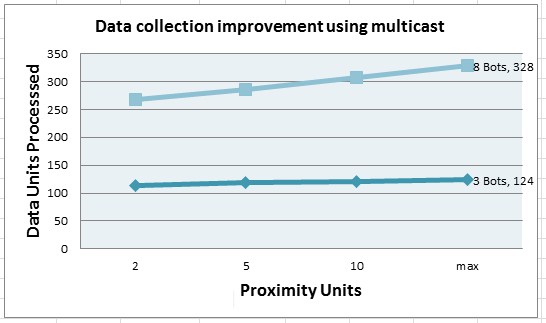
\includegraphics[width=3in]{graph.png}
	\caption{Data Units processed vs Proximity Units.}
	\end{center}
\end{figure}

This same data can be since as percentages of the total data that would have been processed in a conventional system:

%table 2
%\begin{table}
\begin{center}
    \begin{tabular}{ | c | c | c |}
    \hline
    Proximity & \multicolumn{2}{|c|}{Data Units} \\
    Criterion & \multicolumn{2}{|c|}{Processed} \\   \cline{2-3} 
     & 3bots & 8 bots        \\ \hline \hline
    2 & 91.13\% & 81.40\%    \\
    5 & 95.16\% & 86.89\%    \\
    10 & 97.58\% & 93.0\%    \\
    max & 100\% & 100\%	     \\
    \hline
    \end{tabular}
\end{center}
%\caption{Data Units processed as percentage of total.}
%\end{table}

\subsection{Simulation conclusions}
The data is not enough to be conclusive, but the testbench provides a further starting point for analysis, as more robots are included in the simulation and eventually more obstacles and a bigger grid. 
Simulation improvements
There are several improvements that can be explored in new simulation:
\begin{itemize}
\item	The number of robots can be incremented to more significant sized swarms, were data collection inferences can be made with bigger sample sets of robots
\item	The grid size can be incremented and more obstacles included
\item	With a bigger grid and more robots, the probability of robot interactions can increment, such that the proximity criterion can be varied with other than minimal units
\item	More criterion can be included in the multicast selection algorithm (the algorithm that choses which multicast groups to subscribe to) other than proximity. 
\item	The simulation environment can have more significant variables that approach real life characteristics of a robot swarm, such as visibility, robot types, wind, etc.
\item	Opportunity insert different robot types, to create a better swarm eco-system, to improve network behavior such as search, base and relay robots as introduce in \cite{IG5}.
\end{itemize}

\section{Conclusions}

From the research collected in section I and the practical experiment demonstrated in section II we can draw up the following conclusions:


\begin{enumerate}
\item The Mcast protocol can be used to reduce the amount of information being conveyed by the robots. Data collection rates are minimized by the subscription to an Mcast groups to obtain information of interest.

\item A real-time solution is needed to tackle the many critical aspects of the design. One of such aspects is the collision avoidance mechanism. Even if this is not the only activity a robot of this class can perform, the need to perform this task is, by itself, reason enough to use a real-time solution.

\item The nature of the arriving tasks are sporadic and unpredictable. The arrival of tasks depends of a number variables including

\begin{itemize}
\item The distance and trajectory it is heading.
\item The speed with which it is moving.
\item The number of robots in it's vicinity.
\item The number and size of the obstacles.
\end{itemize}

\item The more channels of communication a robot ha access to, the more information it has to take better decisions but at the same time, the more information it has to process, risking missing the deadline for some tasks.

\item There is potential demand in the future for such systems. As robot swarm technologies continues to evolve, the availability of these systems will increase and we will see more and more applications being made for it.

\item There is huge area for improvement in swarm robotics real-time paradigms. If we compare it to the personal computer industry, this is at it's infant stage.

\item Aspects of classic RTOS concepts and scheduling mechanisms can be applied. Future projects may include implementing a hybrid RM (Rate Monotonic) and a EDF (Earliest Deadline First) scheduler inside the kernel and test under what circumstances one is preferred over the other.

\end{enumerate}

While the swarm robotics industry has yet to take off, it poses many challenges in making these systems robust and reliable. A relatively simple and practical experiment using simulated models can prove this point.
For the RTOS community, this presents many rooms for improvements on the current scheduling paradigms and opens a door for new and exciting problems to solve. As we continue to thrive for more speed and intelligence in the robot design, the prospect of seeing a comeback of the machines swarms in a not so distant future is getting closer and closer with each passing day.

%Acknowledgements
\section{Acknowledgment}

%Reference
\ifCLASSOPTIONcaptionsoff
  \newpage
\fi
\begin{thebibliography}{1}

\bibitem{YS1}
Sam Byford, The Verge, \emph{Google Self Driving Cars}, "http://www.theverge.com/2012/12/23/3797260/self-driving-cars-automated-vehicles", 12-23-2012.

\bibitem{YS2}
Alanna Durkin, \emph{Robot Swarm}, "http://adurkin.weebly.com/1/post/2013/04/robot-swarm.html", Apr 8 2012.

\bibitem{YS3.5}
Carlo Ratti, Assaf Biderman, Luigi Farrauto, \emph{Seaswarm}, "http://senseable.mit.edu/seaswarm/", 2013.

\bibitem{YS3.6}
Joseph L. Flatley, \emph{MIT Seaswarm autonomous robots coming soon to an oil spill near you},
"http://www.engadget.com/2010/08/27/mit-seaswarm-autonomous-robots-coming-soon-to-an-oil-spill-near/", Aug 27 2010.

\bibitem{YS3}
John A. Stankovic, Department of Computer Science, University of Massachusetts,\emph{Real-Time Computing}, Amherst MA, April 16, 1992.

\bibitem{HH1}
Xing Jin and Lin Bai and Yuefeng Ji and Yongmei Sun,
Semantics, Knowledge and Grid, 2008. SKG '08. Fourth International Conference on, \emph{Probability Convergence based Particle Swarm Optimization for Multiple Constrained QoS Multicast Routing},
2008, pages 412-415,

\bibitem{HH2}
Jin Lu and Dongfeng Zhao and Zhenzhou An and Wenxue Ran,
Computer Science and Network Technology (ICCSNT), 2011 International Conference on, \emph{Family particle swarm optimization for QoS multicast routing in Ad hoc},
2011,volume 3, pages 1699-1702,

\bibitem{HH4}
Tan Ying and Xue Songdong and Zeng Jianchao and Pan Jengshyang and Pan Tienszu,
Information and Automation (ICIA), 2010 IEEE International Conference on, \emph{Effects of algorithmic parameters on swarm robotic search},
2010, pages 87-92,

\bibitem{HH5} 
Sujit, P. B. and Lucani, D.E. and Sousa, J.B.,
journal=Selected Areas in Communications, IEEE Journal on, \emph{Bridging Cooperative Sensing and Route Planning of Autonomous Vehicles},
2012, pages 912-922,
\bibitem{HH6} 
John Lehoczy, Lui Sha and Ye Ding,
\emph{The Rate Monotonic Scheduling Algorithm: Exact Characterization and Average Case Behavior},
1990

\bibitem{IG1}
He Deng-xu; Zhu Hua-Zheng; Liu Gui-qing, \emph{"Glowworm swarm optimization algorithm for solving multi-constrained QoS multicast routing problem,"} Computational Intelligence and Security (CIS), 2011 Seventh International Conference on , vol., no., pp.66,70, 3-4 Dec. 2011
doi: 10.1109/CIS.2011.23

\bibitem{IG2}
Jin Lu; Dongfeng Zhao; Zhenzhou An; Wenxue Ran, \emph{"Family particle swarm optimization for QoS multicast routing in Ad hoc,"} Computer Science and Network Technology (ICCSNT), 2011 International Conference on , vol.3, no., pp.1699,1702, 24-26 Dec. 2011

\bibitem{IG3}
Chun-bo Liu; Hui-jin Wang; Zhi-ping Luo; Xiu-qin Yu; Li-hua Liu, \emph{"QoS Multicast Routing Problem Based on Artificial Fish-Swarm Algorithm,"} Education Technology and Computer Science, 2009. ETCS '09. First International Workshop on , vol.2, no., pp.814,817, 7-8 March 2009

\bibitem{IG4}
Al-Holou, N.; Booth, K.K.; Yaprak, E., \emph{"Using computer network simulation tools as supplements to computer network curriculum,"} Frontiers in Education Conference, 2000. FIE 2000. 30th Annual , vol.2, no., pp.S2C/13,S2C/16 vol.2, 2000
doi: 10.1109/FIE.2000.896644

\bibitem{IG5}
Jong Sun Kim; Myung Hwan Tak; Young Hoon Joo; Young Jo Cho; Chang Eun Lee; Sang Hoon Ji, \emph{"Behavior control for the swarm robots with network connectivity,"} Ubiquitous Robots and Ambient Intelligence (URAI), 2012 9th International Conference on , vol., no., pp.337,340, 26-28 Nov. 2012
doi: 10.1109/URAI.2012.6463009

\bibitem{IG6}
Mao Yang; Zongchun Liu, \emph{"Control of collision avoidance for swarm robots foraging in complex environment,"} Intelligent Control and Information Processing (ICICIP), 2012 Third International Conference on , vol., no., pp.525,530, 15-17 July 20127

\bibitem{IG7}
V. Gazi and K. M. Passino, \emph{“A class of repulsion/attraction forces for stable swarm aggregations,”} Int. J. Control, vol. 77, no. 18, pp.  1567–1579, 2004

\bibitem{IG8}
Zongchun Liu; Yantao Tian; Mao Yang, \emph{"Behavior analysis in free space and obstacle environment of swarm robot systems based on vicsek model,"} Advanced Computer Control (ICACC), 2010 2nd International Conference on , vol.1, no., pp.224,229, 27-29 March 2010

\bibitem{IG9}
Sharma, R.; Ghose, D., \emph{"Swarm Intelligence based Collision Avoidance Between Realistically Modelled UAV Clusters,"} American Control Conference, 2007. ACC '07 , vol., no., pp.3892,3897, 9-13 July 2007

\bibitem{IG10}
Guohua Ye; Wang, H.O.; Tanaka, K.; Zhi-Hong Guan, \emph{"Managing group behaviors in swarm systems by associations,"} American Control Conference, 2006 , vol., no., pp.8 pp.,, 14-16 June 2006
\end{thebibliography}
\end{document}
